\documentclass[12pt, titlepage]{article}

\usepackage{graphicx}
\graphicspath{ {./images/} }
\usepackage{booktabs}
\usepackage{tabularx}
\usepackage{float}
\usepackage{hyperref}
\usepackage{multirow}
\hypersetup{
    colorlinks,
    citecolor=black,
    filecolor=black,
    linkcolor=red,
    urlcolor=blue
}
\usepackage[round]{natbib}

\title{SE 3XA3: Module Guide\\Euneva}

\author{Team 9, Euneva
		\\ Mehta, Jash - mehtaj8
		\\ Sharma, Aditya - shara24
		\\ Ren, Zackary - renx11
}

\date{\today}
\begin{document}

\maketitle

\pagenumbering{roman}
\tableofcontents
\listoftables
\listoffigures

\begin{table}[bp]
\begin{tabularx}{\textwidth}{p{3cm}p{2cm}X}
\toprule {\bf Date} & {\bf Version} & {\bf Notes}\\
\midrule
17/03/2021 & 1.0 & Initial version of Module Guide\\
\bottomrule
\end{tabularx}
\caption{\bf Revision History}
\end{table}

\newpage

\pagenumbering{arabic}

\section{Introduction}

\subsection{Overview}
The goal of this project is to create a To-Do list software capable of collecting updated assignment and quiz information from Avenue to Learn, and displaying this information in an organized manner. This would allow students to keep track of upcoming assignments and quizzes without having to search from class to class. The current To-Do list software is not capable of scraping Avenue to Learn, therefore the software is a very basic rendition of a To-Do list. This document aims to translate the functional and non-functional requirements as seen in the SRS into a direct programming scenario. This document outlines how the behaviour desired in the SRS will be implemented into the code of the game.

\subsection{Scope}
The final version of Euneva will implement the Avenue to Learn web scraping functionality as well as display the information in an organized and comprehensible manner.

\subsection{Purpose}
The purpose of this document is to provide a written, organized representation between the code design and the requirements. The software being developed has many working parts that all work simultaneously to create the desired functionality. As a result, this document will outline how the modules must interact and function, allowing the current development team to keep track of individual modules, as well as provide a map to future developers.



\section{Anticipated and Unlikely Changes}
This section lists possible changes to the system. According to the likeliness of the change, the possible changes are classified into two categories. Anticipated changes are listed in Section 2.1, and unlikely changes are listed in Section 2.2

\subsection{Anticipated Changes}
Anticipated changes are the source of the information that is to be hidden inside the modules. Ideally, changing one of the anticipated changes will only require changing the one module.\\

\begin{description}
    \item[\textbf{AC1}]: The platforms and devices on which the software is running.
    \item[\textbf{AC2}]: The appearance of the user interface.
    \item[\textbf{AC3}]: The user experience and flow through the app.
\end{description}

\subsection{Unlikely Changes}
The module design should be as general as possible. However, a general system is more complex. Sometimes this complexity is not necessary. Fixing some design decisions at the system architecture stage can simplify the software design. If these decisions should later need to be changed, then many parts of the design will potentially need to be modified. Hence, it is not intended that these decisions will be changed.\\

\begin{description}
    \item[\textbf{UC1}]: Currently the scraping functionality is based on the latest release of Avenue to Learn, therefore if the website being scraped is changed, then the scraping functionality would have to be re-designed.
    \item[\textbf{UC2}]: Converting the application from a Model View Controller architecture to a different architectural style.
\end{description}

\section{Module Hierarchy}
This section presents an overview of the module design. Table 1 describes the modules in a hierarchy. The modules listed as leaves in the hierarchy tree are the modules that will actually be implemented. \\

\begin{description}
    \item[\textbf{M1}]: GUI Module.
    \item[\textbf{M2}]: Login Module
    \item[\textbf{M3}]: Filter Courses Module.
    \item[\textbf{M4}]: Assignment Information Module.
    \item[\textbf{M5}]: Quiz Information Module.
    \item[\textbf{M6}]: Filtering Module. 
\end{description}

\begin{table}[h!]
    \centering
    \begin{tabular}{p{0.4\textwidth} p{0.7\textwidth}}
        \toprule
        \textbf{Level 1} & \textbf{Level 2}\\
        \midrule
        
        {Hardware-Hiding Module} & GUI Module \\
        \midrule
        
        \multirow{4}{0.3\textwidth}{Behaviour-Hiding Module} & Login Module\\
        & Assignment Information Module\\
        & Quiz Information Module\\
        & Filtering Module\\
        \midrule
        
        \multirow{1} {0.35\textwidth}{Software Decision Module} & {Filter Courses Module}\\
        \bottomrule
        
    \end{tabular}
    \caption{Module Hierarchy}
\end{table}


\section{Connection Between Requirements and Design}
The design of the system is intended to satisfy the requirements developed in the SRS. In this stage, the system is decomposed into modules. The connection between requirements and modules is listed in Table 3.

\section{Module Decomposition}
\subsection{Hardware Hiding Modules}
\begin{description}
    \item[\textbf{Secrets:}] The data structures and algorithms used to implement the virtual hardware.
    \item[\textbf{Services:}] Serves as a virtual hardware used by the rest of the system. This module provides the interface between the hardware and the software. So, the system can use it to display outputs or accept inputs.
    \item[\textbf{Implemented By:}] OS
\end{description}

\subsubsection{GUI Module (M1)}
\begin{description}
    \item[\textbf{Secrets:}] Required behaviour of the application elements.
    \item[\textbf{Services:}] Includes programs that provide eternally visible behaviour of the system as specified in the software requirements specification (SRS) documents. This module serves as a communication layer between the hardware-hiding  module and the software decision module. The programs in this module will need to change if there are changes in the SRS.
    \item[\textbf{Implemented By:}] Euneva
\end{description}

\subsection{Behaviour-Hiding Module}
\subsubsection{Login Module (M2)}
\begin{description}
    \item[\textbf{Secrets:}] Gathering and using the users input information to log into Avenue to Learn
    \item[\textbf{Services:}] Uses CSS elements to navigate through the website, placing the correct information given by the user into the correct sections of the website.
    \item[\textbf{Implemented By:}] Euneva
\end{description}

\subsubsection{Filter Courses Module (M3)}
\begin{description}
    \item[\textbf{Secrets:}] Filtering the course information for the current semester.
    \item[\textbf{Services:}] Uses CSS elements to navigate through the website, pressing the correct filter tab.
    \item[\textbf{Implemented By:}] Euneva
\end{description}

\subsubsection{Assignment Information Module (M4)}
\begin{description}
    \item[\textbf{Secrets:}] Collects assignment information for every course.
    \item[\textbf{Services:}] Uses CSS elements to navigate through the website, collecting assignment names, due dates, and completion statuses for every course.
    \item[\textbf{Implemented By:}] Euneva
\end{description}

\subsubsection{Quiz Information Module (M5)}
\begin{description}
    \item[\textbf{Secrets:}] Collects quiz information for every course.
    \item[\textbf{Services:}] Uses CSS elements to navigate through the website, collecting quiz names, due dates, and completion statuses for every course.
    \item[\textbf{Implemented By:}] Euneva
\end{description}

\subsection{Software Decision Module}
\subsubsection{Filtering Module (M6)}
\begin{description}
    \item[\textbf{Secrets:}] Filters and combines the collected information, pushing it to the DB.
    \item[\textbf{Services:}] Uses the collected information and filters it for upcoming and incomplete quizzes and assignments, pushing this information to the front end.
    \item[\textbf{Implemented By:}] Euneva
\end{description}


\section{Traceability Matrix}
This section shows two traceability matrices. Between the modules and the requirements, and between the modules and the anticipated changes.


\begin{table}[H]
    \centering
    \begin{tabular}{p{0.5\textwidth} p{0.6\textwidth}}
        \toprule
        \textbf{Req.} & \textbf{Modules}\\
        \midrule
        \textbf{Functional Requirements}\\
        \midrule
        FR1 & M1\\
        FR2 & M1\\
        FR3 & M1\\
        FR4 & M1\\
        FR5 & M1\\
        FR6 & M1\\
        FR7 & M1\\
        FR8 & M2\\
        FR9 & M3\\
        FR10 & M4\\
        FR11 & M5\\
        FR12 & M5\\
        FR13 & M6\\
        \midrule
        \textbf{Non-Functional Requirements}\\
        \midrule
        LFA1 & M1\\
        LFS1 & M1\\
        UHE1 & M1 \\
        UHP1 & M1 \\
        UHU1 & M1 \\
        UHA1 & M1 \\
        PSL1 & M3, M6 \\
        PPA1 &  M3, M6\\ 
        PRA1 & M1, M2 \\
        PRA2 & M1, M2 \\
        PRF1 & M2, M3, M6 \\
        PCR1 & M2 \\
        PSE1 & M3 \\
        EPE1 & M1 \\
        RIAS1 & M1 \\
        RR1 & M1, M2, M3, M4, M5, M6 \\
        \bottomrule
    \end{tabular}
    \caption{Trace Between Requirements and Modules}
\end{table}

\begin{table}[H]
    \centering
    \begin{tabular}{p{0.6\textwidth} p{0.5\textwidth}}
        \toprule
        \textbf{Req.} & \textbf{Modules}\\
        \midrule
        \textbf{Non-Functional Requirements Cont.}\\     
        RR2 & M1 \\
        MSM1 & M1, M2, M3, M4, M5, M6 \\
        MSM2 & M1 \\
        MSM3 & M1, M2, M3, M4, M5, M6 \\
        SR1 & M1, M2, M3, M4, M5, M6 \\
        ADR1 & M1 \\
        AR1 & M1 \\
        AR2 & M1, M2, M3, M4, M5, M6 \\
        IR1 & M1, M2, M3, M4, M5, M6 \\
        PR1 & M2, M3, M4, M5, M6 \\
        PR2 & M2, M3, M4, M5, M6 \\
        CPC1 & M1 \\
        CPC2 & M1 \\
        \bottomrule
    \end{tabular}
    \caption{Trace Between Requirements and Modules Cont.}
\end{table}

\begin{table}[H]
    \centering
    \begin{tabular}{p{0.5\textwidth} p{0.6\textwidth}}
        \toprule
        \textbf{AC} & \textbf{Modules}\\
        \midrule
            AC1 & M1, M2 \\
            AC2 & M1, M2 \\
            AC3 & M1, M2, M3, M4, M5, M6 \\
        \bottomrule
    \end{tabular}
    \caption{Trace Between Anticipated Changes and Modules}
\end{table}

\section{User Hierarchy Between Modules}
As shown by \ref{hierarchyFig}, the graph representing the relationship
between the modules is a directed acyclic graph (DAG). 
The modules have purposely been designed to mimic a tree due to the way
how technologies like React work when rendering information. Simplicity was 
key when developing this product, so we followed a pipelined approach which is why
the module hierarchy is more tree-like rather than graph-like.
 
\begin{figure}[H]
    \centering
    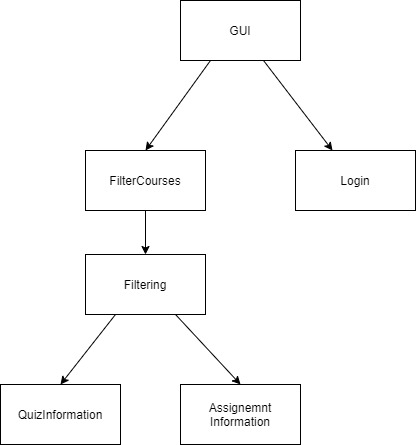
\includegraphics[width=0.7\textwidth]{hierarchy.jpg}
    \caption{Module Use Hierarchy}
    \label{hierarchyFig}
\end{figure}
    

\end{document}
